\chapter{Simulaciones}
\lhead{\emph{Simulaciones}}

En este capítulo se presentan las mediciones y ensayos realizados para estudiar y comparar como se comportan ambos métodos de
calibración, clásica y utilizando acoplamientos mútuos.

La configuración de la antena a utilizar para todos los ensayos está especificada en la tabla \ref{tab:configurationUsed} y 
consta de 70 elementos radiantes. Las especificaciones de las propiedades físicas de cada componente están definidas en la 
tabla \ref{tab:configurationOfComponents}.
\begin{table}[H]
  \footnotesize
  \centering
  \begin{tabular}{|c|c|}
	\hline
	\textbf{Componente de Antena} & \textbf{Configuración} \tabularnewline \hline 
	freq &  1275000000 [Hz] \tabularnewline\hline 
	power & 0 [dB] \tabularnewline \hline 
	phase & 0 [deg] \tabularnewline \hline 
	desiredTxPower & 20 [dB] \tabularnewline \hline 
	desiredRxPower & 0 [dB] \tabularnewline \hline 
	quantityRows & 7 \tabularnewline \hline 
	quantityColumns & 10 \tabularnewline \hline 
	verticalSeparation & 0.2 [m] \tabularnewline \hline 
	hotizontalSeparation & 0.2 [m] \tabularnewline \hline 
	componentSequence & [cable1, psc17, cable1, psc15, cable2, psc12, trm, circulator, cable3, rm] \tabularnewline \hline 
  \end{tabular}
  \caption{Configuración de la antena común para todos los ensayos.}
  \label{tab:configurationUsed}
\end{table}
\begin{table}[H]
  \footnotesize
  \centering
  \begin{tabular}{|c|c|c|}
	\hline
	\textbf{Componente de Antena} & \textbf{Cacarcterísticas físicas} & \textbf{Configuración} \tabularnewline \hline 
	\multirow{2}{*}{cable1} &  attenuation [db] & 0.1\tabularnewline \cline{2-3}
	 & length [m] & 0.45\tabularnewline \hline 
	\multirow{2}{*}{cable2} &  attenuation [db] & 0.1\tabularnewline \cline{2-3}
	 & length [m] & 8\tabularnewline \hline 
	\multirow{2}{*}{cable3} &  attenuation [db] & 0.1\tabularnewline \cline{2-3}
	 & length [m] & 0.5\tabularnewline \hline 
	psc17 & outputPorts & 7\tabularnewline \hline
	psc15 & outputPorts & 5\tabularnewline \hline
	psc12 & outputPorts & 2\tabularnewline \hline
	\multirow{2}{*}{TRM} & gain [db] & 10\tabularnewline \cline{2-3}
	 & phaseShift [deg] & 10\tabularnewline \hline 
	circulator & & \tabularnewline \hline 
	RM & & \tabularnewline \hline 
  \end{tabular}
  \caption{Configuración de las propiedades físicas de cada componente de la antena utilizada en todos los ensayos.}
  \label{tab:configurationOfComponents}
\end{table}
La numeración de los elementos tiene un orden de izquierda a derecha y de forma descendiente, de tal forma que el elemnto cero 
es el superior izquierdo de la antena.

\section{Sin errores}

Los ensayos de esta sección tienen las siguientes caracterísiticas,
\begin{itemize}
	\item Ensayar ambos métodos de calibración con diferentes apuntamientos de la antena.
	\item Los distintos apuntamientos utilizados son: Uniforme, 10 grados en la dirección horizontal y 10 grados en la dirección 
		vertical.
	\item Los componentes de antena no tienen ningún prolema de funcionamiento ni hay desadaptaciones.
	\item No hay errores de calibración.
	\item No hay errores en la señal.
\end{itemize}

\subsection{Utilizando la calibración clásica}
\todo{:D}
\subsection{Utilizando la calibración con acoplamientos mútuos}

En la figura \ref{fig:nonErrorMutual} se puede observar que el método funciona correctamente. La subfigura a muestra un 
apuntamiento de cero grados, la b, de 10 grados en dirección horizontal, y la tercera de 10 grados en dirección vertical.

Se puede verificar que el apuntamiento es el correcto por los defasajes observados, como hay 10 elementos radiantes por fila,
al apuntar verticalmente, cada fila posee un defasaje diferente, es por esta razón que la tercer fila se ve un gráfico estilo 
una escalera con siete escalones (que es la cantidad de columnas de la antena). 
\begin{figure}[H]
	\centering
 	\subfloat[]{
		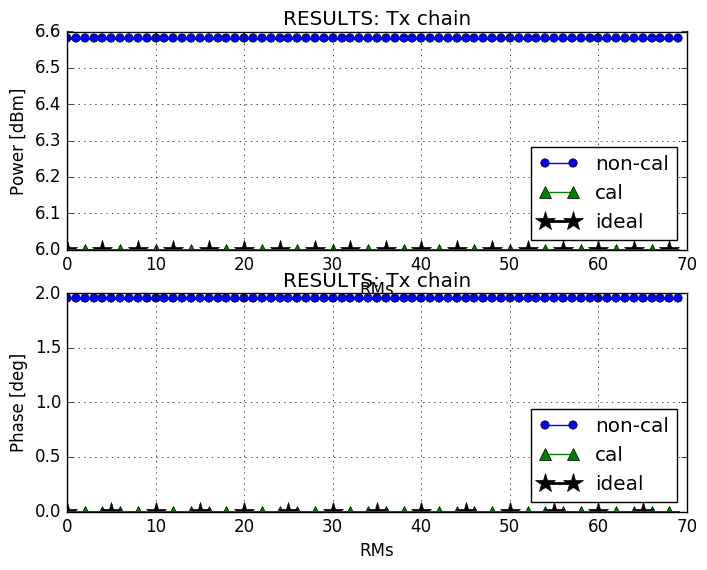
\includegraphics[width=10cm]{gfx/nonErrMutual0deg.png}}
 	
	\subfloat[]{
		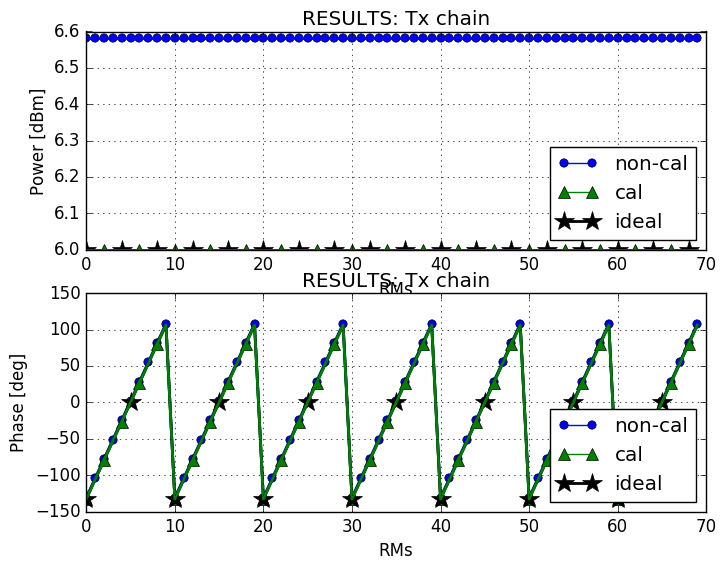
\includegraphics[width=8cm]{gfx/nonErrMutual10degCol.png}}
	\subfloat[]{
		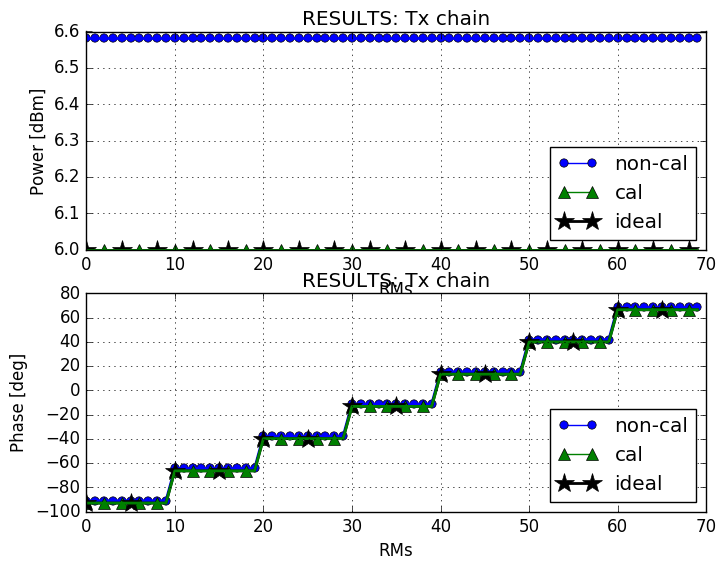
\includegraphics[width=8cm]{gfx/nonErrMutual10degRow.png}}
		\caption{Antena calibrada con distintos apuntamientos utilizando acoplamientos mútuos. (a) 0 grados. (b) 10 grados en 
		dirección horizontal. (c) 10 grados en dirección vertical.}
	\label{fig:nonErrorMutual}
\end{figure}


\section{Rotura de varios TRMs}

Los ensayos de esta sección tienen las siguientes caracterísiticas,
\begin{itemize}
	\item Ensayar ambos métodos de calibración con diferentes apuntamientos de la antena.
	\item Los distintos apuntamientos utilizados son: Uniforme, 10 grados en la dirección horizontal y 10 grados en la dirección 
		vertical.
	\item Salvo tres TRMs que están rotos, el resto de los componentes de antena no tienen ningún prolema de funcionamiento ni 
		desadaptaciones. Las posiciones de los TRMs son: [1,0], [3,4] y [5,5]. La nomenclatura de lectura es [fila, columna] con 
		valores desde 0.
	\item No hay errores de calibración.
	\item No hay errores en la señal.
\end{itemize}

\subsection{Utilizando la calibración clásica}
\todo{:D}
\subsection{Utilizando la calibración con acoplamientos mútuos}

En la figura \ref{fig:deadTRMsMutual} se puede observar que independientemente de que se hayan destruído varios TRMs, el 
método puede calibrar los lazos, obteniendo los valores deseados, tanto de fase como de ganancia del resto de los elementos.
La subfigura (a) muestra un apuntamiento de cero grados, la (b), de 10 grados en dirección horizontal, y la tercera de 10 grados
en dirección vertical.

\begin{figure}[H]
	\centering
 	\subfloat[]{
		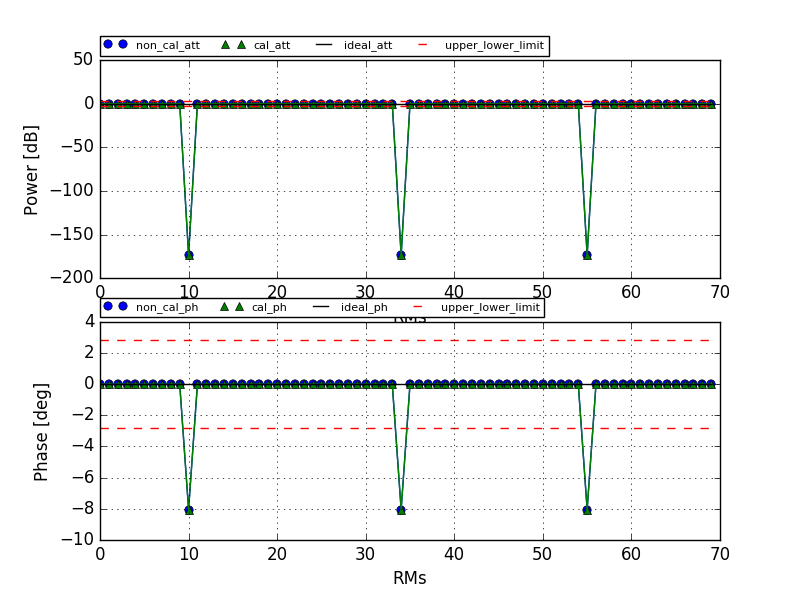
\includegraphics[width=10cm]{gfx/deadTRMsMutual0deg.png}}
 	
	\subfloat[]{
		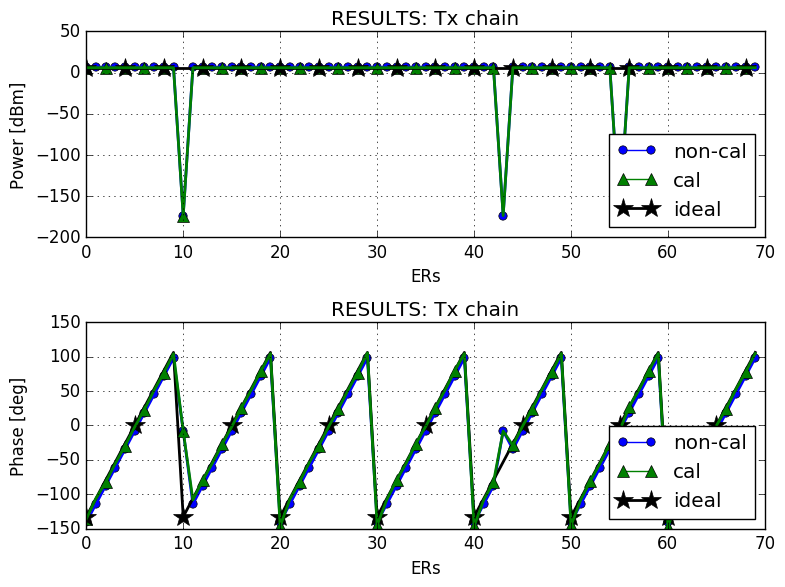
\includegraphics[width=8cm]{gfx/deadTRMsMutual10degCol.png}}
	\subfloat[]{
		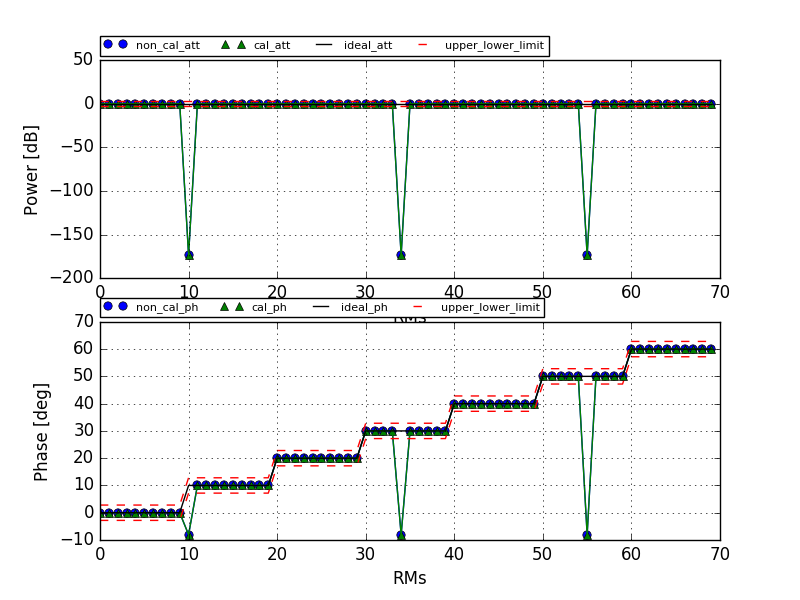
\includegraphics[width=8cm]{gfx/deadTRMsMutual10degRow.png}}
		\caption{Antena calibrada con distintos apuntamientos utilizando acoplamientos mútuos. (a) 0 grados. (b) 10 grados en 
		dirección horizontal. (c) 10 grados en dirección vertical.}
	\label{fig:deadTRMsMutual}
\end{figure}


\section{Errores en comportamiento de componentes de la antena}

Los ensayos de esta sección tienen las siguientes caracterísiticas,
\begin{itemize}
	\item Ensayar ambos métodos de calibración con diferentes apuntamientos de la antena.
	\item Los distintos apuntamientos utilizados son: Uniforme, 10 grados en la dirección horizontal y 10 grados en la dirección 
		vertical.
	\item Hay dispersiones de comportamiento en los siguientes componentes de la antena: circuladores, TRMs, PSCs y RMs. Las 
		magnitudes están especificadas en la tabla \ref{tab:errorReferences}.
		\begin{table}[H]
		  \footnotesize
		  \centering
		  \begin{tabular}{|c|c|}
			\hline
			\textbf{Error de componente} & \textbf{Desvío estandar} \tabularnewline \hline 
			Error de ganancia del circulador &  0.2 [dB] \tabularnewline\hline 
			Error de fase del circulador &  10 [deg] \tabularnewline\hline 
			Error de ganancia del TRM &  0.2 [dB] \tabularnewline\hline 
			Error de fase del TRM &  10 [deg] \tabularnewline\hline 
			Error de ganancia del PSC &  0.1 [dB] \tabularnewline\hline 
			Error de fase del PSC &  10 [deg] \tabularnewline\hline 
		  \end{tabular}
		  \caption{Configuración de los errores de componentes.}
		  \label{tab:errorReferences}
		\end{table}
	\item No hay errores de calibración.
	\item No hay errores en la señal.
\end{itemize}

\subsection{Utilizando la calibración clásica}
\todo{:D}
\subsection{Utilizando la calibración con acoplamientos mútuos}

En la figura \ref{fig:componentErrorsMutual} se puede observar que si bien, en algunos ensayos el método no corrige 
perfectamente la fase por el error agregado de todos los componentes de la RFDN a la vez, en una segunda iteración se logra 
llegar a dicho valor. La subfigura (a) muestra un apuntamiento de cero grados, la (b), de 10 grados en 
dirección horizontal, y la tercera de 10 grados en dirección vertical.

\begin{figure}[H]
	\centering
 	\subfloat[]{
		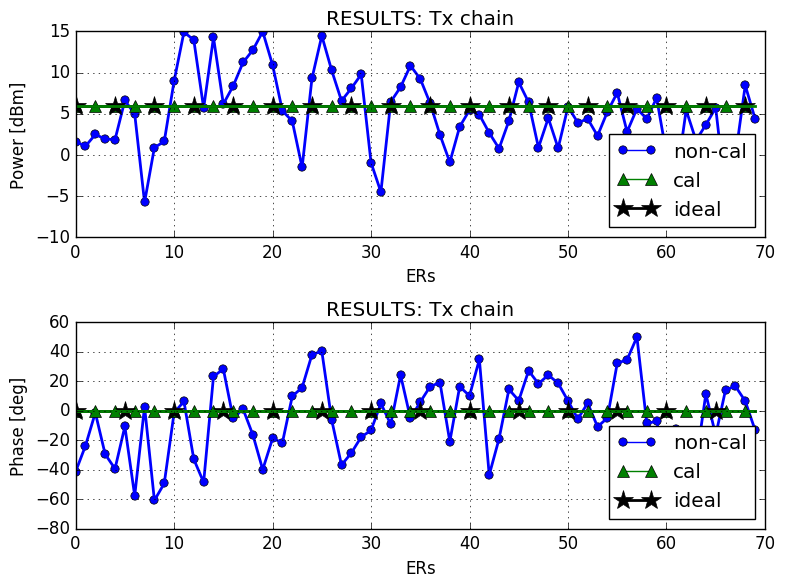
\includegraphics[width=10cm]{gfx/compErrMutual0deg.png}}
 	
	\subfloat[]{
		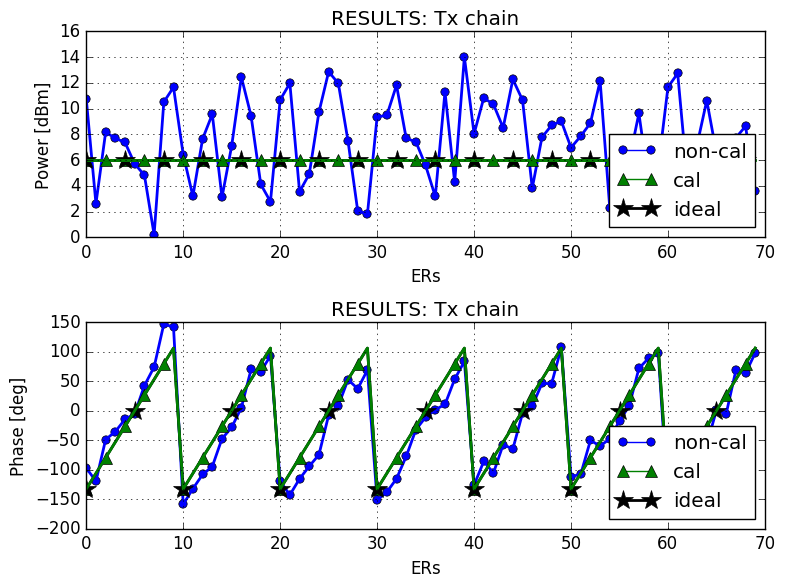
\includegraphics[width=8cm]{gfx/compErrMutual10degCol.png}}
	\subfloat[]{
		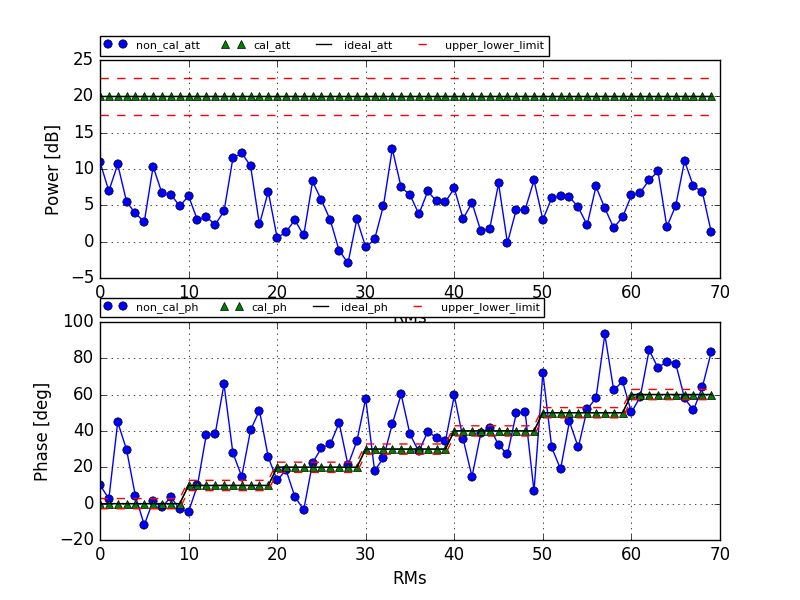
\includegraphics[width=8cm]{gfx/compErrMutual10degRow.png}}
		\caption{Antena calibrada con distintos apuntamientos utilizando acoplamientos mútuos. (a) 0 grados. (b) 10 grados en 
		dirección horizontal. (c) 10 grados en dirección vertical.}
	\label{fig:componentErrorsMutual}
\end{figure}


\section{Errores de ganancia entre pulsos}
\section{Errores de fase entre pulsos}
\section{Error de ganancia de la chirp réplica}

Como la chirp réplica es simplemente utilizada en la calibración clásica, en esta simulación no se podrán comparar 
resultados, pero sirve para determinar que tan robusto es el método para esta clase de erorres.


\section{Error de fase de la chirp réplica}

Como la chirp réplica es simplemente utilizada en la calibración clásica, en esta simulación no se podrán comparar 
resultados, pero sirve para determinar que tan robusto es el método para esta clase de erorres.


\section{Error de fase del Walsh}

Como los códigos walsh son solamente utilizados en la calibración clásica, en esta simulación no se podrán comparar 
resultados, pero sirve para determinar que tan robusto es el método para esta clase de erorres.
